\chapter{Einleitung}
\section{Hintergrund}
Die Chemie im Allgemeinen befasst sich mit den Eigenschaften und Interaktionen
von Molekülen bzw. Atomen. Es ist also von hohem Interesse diese
durch akkurate Modelle zu beschreiben. In der Chemie, wie mit allen
Naturwissenschaften, wurden im Laufe der Geschichte immer genauere Theorien entwickelt.
Im 20. Jahrhundert kam es dann zur Begründung der Computerchemie durch die Einführung zweier 
revolutionärer Gebiete, die der Quantenphysik und der Informatik.
Nun war es nicht nur möglich chemische Systeme auf vorher ungesehene Genauigkeit zu beschreiben,
sondern auch noch quantitative Berechnungen mit Computern an diesen durchzuführen.
Deshalb handelt es sich bei der Computerchemie möglicherweise zukünftig
um eines der nützlichesten Werkzeuge in der Chemie.

\begin{figure}[h]
    \begin{center}
    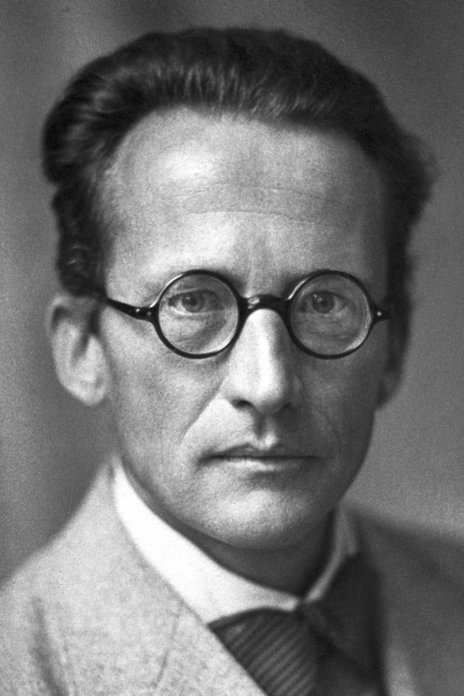
\includegraphics[width=0.25\textwidth]{res/schrodinger.jpg}
    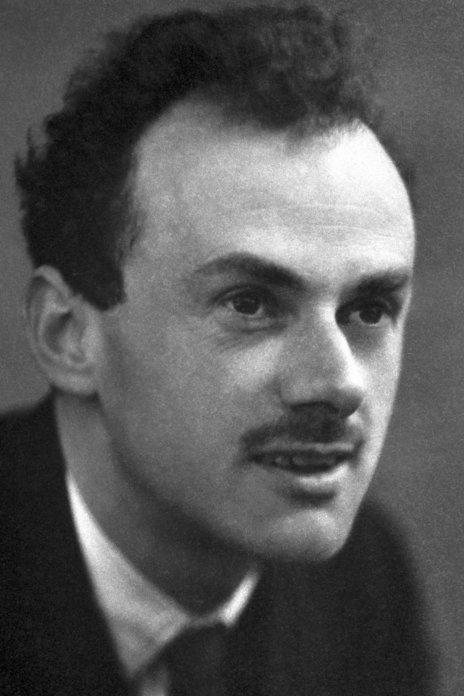
\includegraphics[width=0.25\textwidth]{res/dirac.jpg}
\end{center}
    \caption{Erwin Schrödinger und Paul Adrien Maurice Dirac wurden 1933 mit dem Nobelpreis
    für Physik ausgezeichnet für ihre Entdeckungen im Bezug auf Atomtheorie. \cite{nobel_1933}}
\end{figure}

\section{Ziele}
Wegen der hohen Komplexität und Weitläufigkeit der Computerchemie
kann der Einstieg oft schwierig sein. Aus diesem Grund wird
in dieser Arbeit versucht eine Übersicht der notwendigen Theorie zu geben,
um selber einfache quantenchemische Berechnungen durchzuführen.
Zudem wird noch eine eigene Implementierung
zur Theorie bereitgestellt und besprochen.

Zum Einstieg bietet sich die Berechnung von wohl einer der fundamentalsten Eigenschaften 
eines Moleküls bzw. Atoms an, die Hartree\-/Fock\-/Energie, 
mit dieser können viele Prozesse in der Chemie,
wie Reaktionsabläufe und Molekülstrukturen, erklärt werden.